\documentclass[a4paper,12pt]{article}
%%%%%%%%%%%%%%%%%%%%%%%%%%%%%%%%%%%%%%%%%%%%%%%%%%%%%%%%%%%%%%%%%%%%%%%%%%%%%%%%%%%%%%%%%%%%%%%%%%%%%%%%%%%%%%%%%%%%%%%%%%%%%%%%%%%%%%%%%%%%%%%%%%%%%%%%%%%%%%%%%%%%%%%%%%%%%%%%%%%%%%%%%%%%%%%%%%%%%%%%%%%%%%%%%%%%%%%%%%%%%%%%%%%%%%%%%%%%%%%%%%%%%%%%%%%%
\usepackage{eurosym}
\usepackage{vmargin}
\usepackage{amsmath}
\usepackage{graphics}
\usepackage{epsfig}
\usepackage{enumerate}
\usepackage{multicol}
\usepackage{subfigure}
\usepackage{fancyhdr}
\usepackage{listings}
\usepackage{framed}
\usepackage{graphicx}
\usepackage{amsmath}
\usepackage{chngpage}
%\usepackage{bigints}

\usepackage{vmargin}
% left top textwidth textheight headheight
% headsep footheight footskip
\setmargins{2.0cm}{2.5cm}{16 cm}{22cm}{0.5cm}{0cm}{1cm}{1cm}
\renewcommand{\baselinestretch}{1.3}

\setcounter{MaxMatrixCols}{10}

\begin{document}
\large 

\noindent Suppose X has survival function defined by


\[ S_{o}(X) = \frac{1}{10} (100 - x)^{\frac{1}{2}} \mbox { for }0 \leq x \leq 100.\]

\noindent Create a function for survival model in R and then find the probability of:

\begin{enumerate}[(a)]
    \item a new born surviving till age 65.
    \item 10 year old surviving till 95.
    \item a new born die between the ages 65 and 70 years.
\end{enumerate}


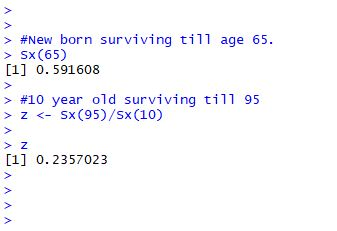
\includegraphics[]{00-B2/images/Mortality_1.JPG}

\begin{framed} \begin{verbatim}
#Define a function for S(x).

Sx <- function(x){
 0.1*(100-x)^(1/2)
 }


#New born surviving till age 65.
Sx(65)



\end{verbatim}\end{framed}


0.591607978309962



\begin{framed} \begin{verbatim}

#10 year old surviving till 95
z<-Sx(95)/Sx(10)
z

\end{verbatim}\end{framed}


0.235702260395516



\begin{framed} \begin{verbatim}
#New born dying between the age of 65-70 years
x<-Sx(65)-Sx(70)
x

\end{verbatim}\end{framed}


0.0438854208047954


%%%%%%%%%%%%%%%%%%%%%%%%%%%%%%%%%%%%%
\newpage 

Create a mortality table q(x) using the survival function above for ages
\[1,5,10,15,20,\ldots 85,90,95,96,97,98.\]


\begin{framed} \begin{verbatim}
age<-c(1,seq(5,95,by=5),seq(96,98,by=1))
qx<-function(x){
1-(Sx(x+1)/Sx(x))}
mortality.table<-data.frame(age)
mortality.table$q.x<-round(qx(mortality.table$age),10)
\end{verbatim}\end{framed}

\newpage 
\begin{framed} \begin{verbatim}
mortality.table
\end{verbatim}\end{framed}

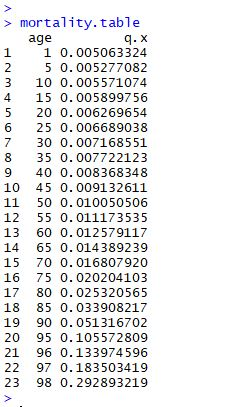
\includegraphics[scale=1.5]{00-B2/images/Mortality_2_table.JPG}


%%%%%%%%%%%%%%%%%%%%%%%%
\newpage
\subsection*{Exercise 3}
\noident Suppose Mu(x) has the following function:

\[ \mu_{x} = \frac{1}{2(100-x)} \mbox { for }0 \leq x \leq 100.\]

\noindent Use the approximation $q_x = 1 - exp(-\mu_{x}(x+1/2)$ to identify \texttt{qx} of all ages in table
\[1,5,10,15,20..........85,90,95,96,97,98. \]
\end{verbatim}\end{framed}


\begin{framed} \begin{verbatim}
#Define a function for Mu(x).
mu<-function(x){
1/(2*(100-x))}
# Calculate qx for each age using approximation
qx1<-function(x){
1-exp(-mu(x+1/2))}
mortality.table$q.x1<-round(qx1(mortality.table$age),10)
mortality.table


\end{verbatim}
\end{framed}
\newpage 
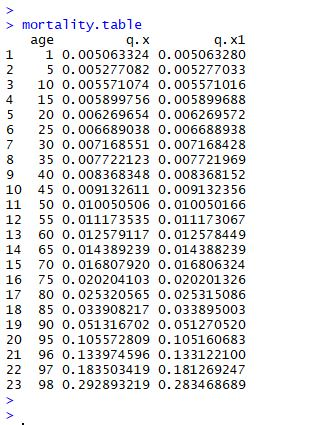
\includegraphics[scale=1.4]{00-B2/images/Mortality_3_table_2.JPG}


%%%%%%%%%%%%%%%%%%%%%%%%
\newpage
\subsection*{Exercise 4}
\noindent Plot a graph compare the \texttt{qx} derived from the survival function in Exercise 1 (in red color)
and function of \texttt{Mu.x} in Exercise 3 (in blue color).


\begin{framed} \begin{verbatim}
# Ploting qx and qx1 using the line graph.

plot( seq(1,98), qx(seq(1,98)) ,
	pch=17,
	col="Red") 

lines( seq(1,98), qx1(seq(1,98)) ,
	col="Blue")
\end{verbatim}\end{framed}

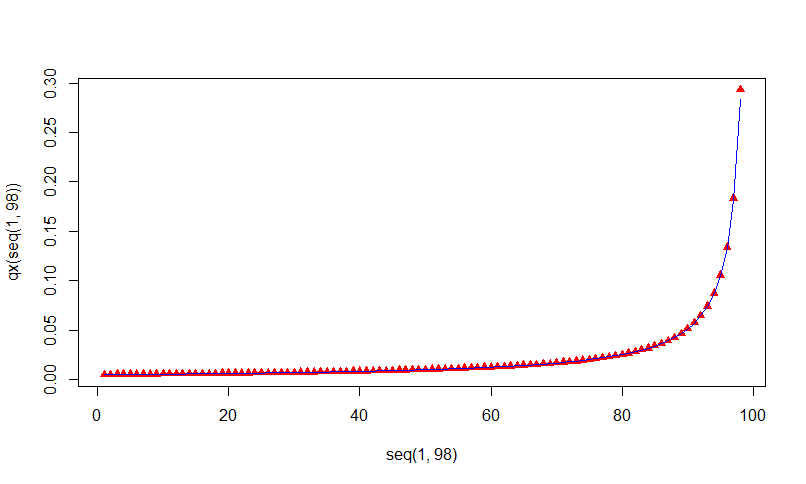
\includegraphics[scale=0.6]{00-B2/images/Mortality_4_Curve.png}

\newpage 



Please comment if the qx derived from survival function is similar with the qx derived
using the Mu function. Please support your answer basis the relationship between the
two functions.



%%%%%%%%%%%%%%%%%%%%%%%%
\newpage
\subsection*{Exercise 5}
v) # Commentary on the graph.
Below is the relationship between the survival function S 0 (x) and hazard function μ x :
S 0 (x) = exp[-integral(μ x (t) dt]
.......(1)


\begin{itemize}
    \item The survival function S 0 (x) above is defined as:
δ/δτ [log (S 0 (x)] = μ x = 1 / 2(100-x)
    \item Deriving μ x using the above relationship in (1), we get the same function for μ x as specified in part (c) and
hence creating mortality table using either survival function or hazard function shall give the same result.
    \item There are minor differences in the graph of qx and that is purely due to the approximation assumed in part (c)
\end{itemize}


\end{document}
